\documentclass[conference]{IEEEtran}
\IEEEoverridecommandlockouts
% The preceding line is only needed to identify funding in the first footnote. If that is unneeded, please comment it out.
\usepackage{cite}
\usepackage{amsmath,amssymb,amsfonts}
\usepackage[T1]{fontenc}
\usepackage{algorithmic}
\usepackage{amsmath,amssymb,amsfonts}
\usepackage{graphicx}
\usepackage{subfig}
\usepackage{textcomp}
\usepackage{xcolor}
\usepackage{listings}
\usepackage{hyperref}
\def\BibTeX{{\rm B\kern-.05em{\sc i\kern-.025em b}\kern-.08em
    T\kern-.1667em\lower.7ex\hbox{E}\kern-.125emX}}
\begin{document}

\title{MACHINE LEARNING APPROACH FOR THE PREDICTION OF THE STATUS OF TANZANIAN WELLS [COMP4030 CW2 - Data Science and Machine Learning]
}

\author{\IEEEauthorblockN{*Thomas Cotter}
\IEEEauthorblockA{\textit{Computer Science} \\
\textit{University of Nottingham}\\
Nottingham, England\\
psytc8@nottingham.ac.uk}
\and
\IEEEauthorblockN{*Loo Yang Shen Jason}
\IEEEauthorblockA{\textit{Computer Science} \\
\textit{University of Nottingham}\\
Nottingham, England \\
hfyyl5@nottingham.ac.uk}
}

\maketitle

\begin{abstract}
  This paper details our approaches and results for the COMP4030 CW2. We have used a number of machine learning algorithms in order to predict the status ('Functional', 'Functional - Needs Repair' \& 'Non-Functional') of water wells in Tanzania. This is important as not only does knowing the status of the well help keep the total percentage of functioning wells higher, but it also allows for more effective spending from the government as they no longer would have to send workers out to check the status of the well. Our results suggested that the most important features were \textbf{ADD RESULTS}, and the best classification model as \textbf{ADD RESULTS}
\end{abstract}

\begin{IEEEkeywords}
  Machine Learning, Data Science, Classification
\end{IEEEkeywords}

\section{Introduction}

This section will provide an introduction to the dataset and the research questions we have attempted to solve.

\subsection{Research Questions}

We have decided that our research question will be: 

\textbf{What factors are most important for determining the status of a well, and how accurately can we classify wells based on these features?}. 

We choose this question because we are interested in the factors that determine the status of a well, and using ML to try to classify these wells into 1 of 3 classes: Functional, Non-Functional \& Functional Needs Repair. From this question, we can think about some follow-up questions. These could include:
    \begin{itemize}
        \item How does the accuracy of the classification model vary with different feature sets and classification algorithms?
        \item Could we use our results to ensure that wells are built and repaired so that fewer wells are non-functional?
    \end{itemize}

\textbf{Perhaps we could also include a section on the importance of this research or some more dicussion on the research questions?}

\subsection{Dataset}

We will be using the dataset from the Tanzanian Ministry of Water, which contains information on the status of wells in Tanzania to answer our research question. This dataset has 59400 rows, with 40 different features. These 40 features could be broken down into three subgroups which hold information regarding: a) Geographic Location of the Wells. b) Management of the wells. and c) Water Condition of the wells. The dataset is originally split into 2 different files, one for labels and one for the actual data. These can be merged easily with pandas through left join on the "ID" column. 


We have done a range of statistical analysis on the dataset, including the value counts and graphical representations of each feature. This can be seen here \url{https://github.com/tomcotter7/dma-project/blob/main/Data%20Understanding%20%26%20Statistical%20Analysis.ipynb}. This will also be discussed further in the Results section.

Fig. \ref{fig:status_groups} shows the distribution of the target variable, which is the status of the well. We can see from this that we might need to oversample the 'functional needs repair' class.

\begin{figure}[h]
    \centering
    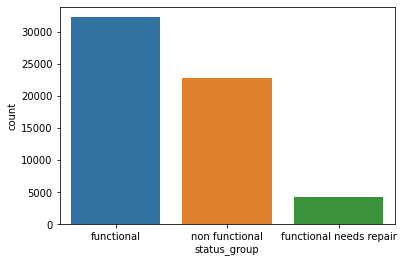
\includegraphics[scale=0.5]{figures/status_groups.png}
    \caption{Distribution of the target variable}
    \label{fig:status_groups}
\end{figure}

\section{Literature Review}

In this section, we review the relevant literature on predicting machine failure, with a focus on studies that have used similar datasets to Pump It Up. Prediciting machine failure is an important area of reasearch, as it has the potential to reduce downtime and maintenance costs. Some machines may be part of a critical infrastructure, so preventing them from failure is of upmost importance.

One study by Pathak et al. (2023) \cite{pathak2023pump} compared the performance of TabNet, a sequential attentive classification architecutre designed for tabular data, and tree-based approaches such as XBBoost. They found that TabNet outpeformed XGBoost, boasting an 83\% accuracy compared to XGBoosts 78\%. TabNet makes use of Transformers, a machine learning algorithm which uses self-attention to differentially weight the significance of each part of the input. A point of note is that TabNet does not require feature engineering to perform at these standards. While TabNet is an interesting solution, we have not used it in our report, as our primary goal was to showcase an end-to-end machine learning solution, and this includes feature enginering.

Jabeur et al \cite{JABEUR2021} conducted a detailed review of different algorithms for predicting financial distress, including, SVMs, Neural Networks, RandomForest, XGBoost \& CatBoost. They found that the ensemble methods worked the most effectively (RandomForest, XGBoost \& CatBoost). Ensemble methods combine multiple models in order to improve accuracy. 

Similary, Mahabub \cite{Mahabub2020} investigated the effectiveness of ensemble methods to detect fake news. They found that combining different classification methods into a Ensemble Voting Classifier produced the best results.

Finally, Celikmih et al \cite{celikmih2020} used classification models to predict the failure of aircraft equipment and employed the ReliefF feature selection algorithm. This algorithm estimates feature weights iteratively, according to their ability to make a distinction between neighboring models. They used this to select the best subset of features to feed into their classification model, resulting in the best performance.

\section{Methodology}

\section{Results}

\subsection{Data Analysis}

\subsection{Data Preprocessing}

\subsection{Classification}

\section{Discussion}

\section{Conclusion}

\bibliographystyle{plain}
\bibliography{refs}

\end{document}


